\section{Introduction}
\label{introduction}


The last 20 years have seen a massive increase in flows from \textit{active investing} strategies trying to outperform a given benchmark index, towards \textit{passive index investing} strategies trying to replicate a benchmark index \parencite{jpmorgan-exchange-traded-funds-etfs}. In this era, new index investing methods have emerged \parencite{jorion-enhanced-index-funds-and-tracking-error-optimization}. \textit{Enhanced index investing} is one such method, seeking to replicate the benchmark risk while outperforming the benchmark return \parencite{investopedia-passive-and-active-funds}. In this pursuit, enhanced index funds have found positive excess returns from exploiting the price effects of stocks being added or deleted from their benchmark index \parencite{nbim-investing-in-equities}. These price effects were first observed by \textcite{shleifer-do-demand-curves-for-stocks-slope-down} on the benchmark index S\&P 500, and subsequently named the S\&P phenomenon, or the \textit{index effect}. Since the discovery of the index effect by \textcite{shleifer-do-demand-curves-for-stocks-slope-down}, it has been investigated further \parencite{lynch-new-evidence-s&p-500}, and observed on other benchmark indices \parencite{afego-effects-of-changes-in-stock-index-composition}. In \autoref{fig:index-effect-osebx} we illustrate the average price movement of additions and deletions from 2002 to 2023 on the Oslo Stock Exchange Benchmark Index (OSEBX). 
\vspace{-1.3em}
\begin{figure}[H]
    \centering
    \makebox[\linewidth][c]{\hspace{-0.6em}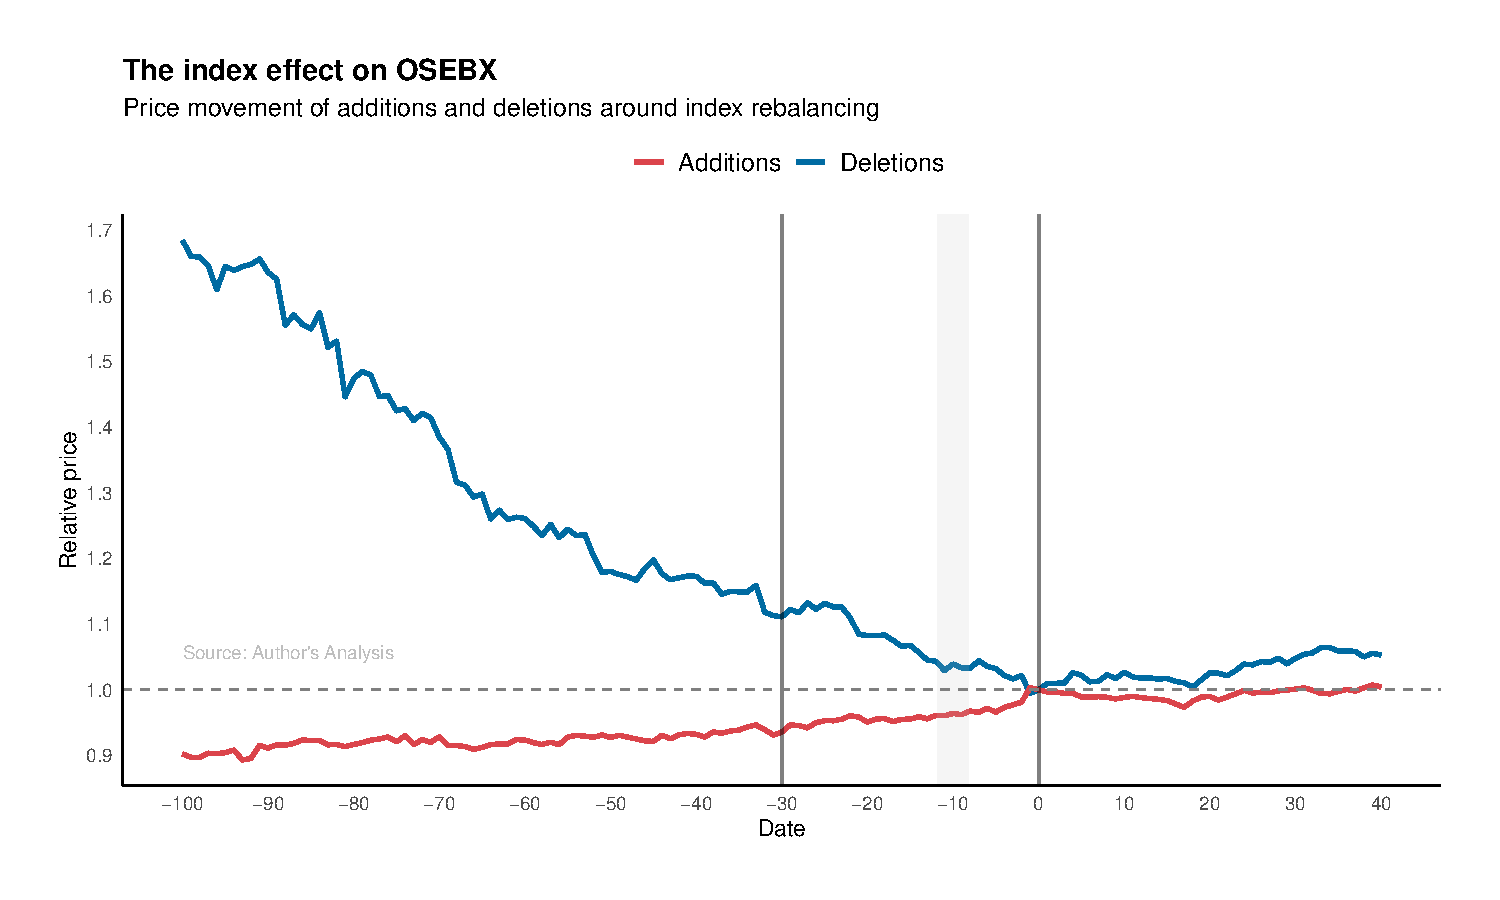
\includegraphics[width=1.0\textwidth]{images/index_plot_updated.pdf}}
    \caption{The Index Effect on OSEBX}
    \subcaption*{
     Illustration of aggregated relative price movements to the first effective day (day 0) with additions and deletions for OSEBX from 2002 to 2023. Day 0 represents the first day after the effective date (ED). The announcement date is typically 14 days ahead of the ED, and the data cutoff date (the day data is extracted for each company, which determines the index composition) is about 30 days in advance of the ED. The figure is generated using price data from Bloomberg.}
    \label{fig:index-effect-osebx}
\end{figure}

Similar to \textcite{shleifer-do-demand-curves-for-stocks-slope-down}, \autoref{fig:index-effect-osebx} shows that the stock price of additions typically increases in the period before being added to the benchmark index, with the equivalent opposite effect for deletions. There have also been some master's theses indicating the existence of such an effect on OSEBX, among those by \textcite{cbs-thesis-price-and-volume-effects-osebx} and \textcite{nhh-thesis-exploiting-the-index-effect-to-extract-alpha}. In short, \autoref{fig:index-effect-osebx} shows our illustration of the index effect on OSEBX since 2002. 

In March and September of each year, Euronext decides which companies should be on OSEBX. This event is guided by three dates, the cut-off date (CD), announcement date (AD), and effective date (ED) \parencite{OSEBX-rule-book}. The CD represents the day Euronext extracts data to use for the index rebalancing event. The index composition is announced on AD and implemented on ED. There are typically a few weeks between CD-AD and AD-ED. \autoref{fig:returns-for-additions-and-deletions-on-osebx} illustrate returns on OSEBX additions and deletions in the 50 days surrounding ED, indicating abnormal returns on ED.  

\vspace{-0.9em}
\begin{figure}[h]
    \centering
    
    \makebox[\linewidth][c]{\hspace{-0.6em}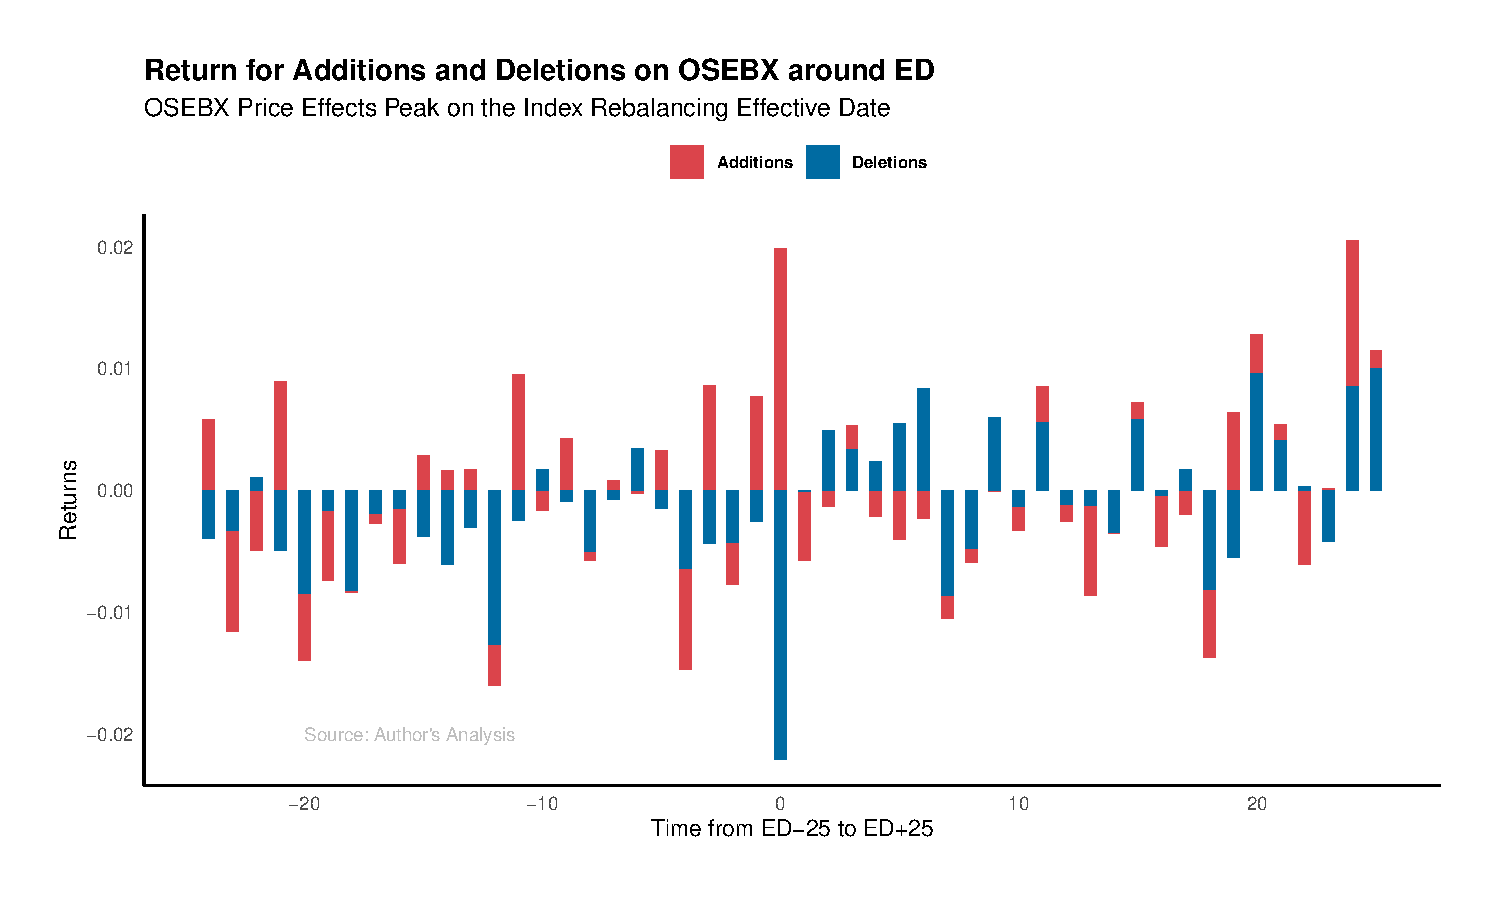
\includegraphics[width=1.06\textwidth]{images/retplot.pdf}}
    \caption{{Return for Additions and Deletions on OSEBX around ED}}
    \subcaption*{We illustrate the aggregated returns for additions and deletions to OSEBX from 2002 to 2023. The figure indicates abnormal returns for both additions and deletions on ED. The return on additions/deletions seems to rise/fall before ED, and somewhat readjust after ED.}
    \label{fig:returns-for-additions-and-deletions-on-osebx}
\end{figure}

In this thesis, we use machine learning (ML) to predict upcoming 
\textit{additions} and \textit{deletions} to OSEBX ahead of AD. Additions are companies not currently on OSEBX, which enter from one period to the next, and deletions are companies exiting OSEBX from one period to the next. By predicting before the AD, we can potentially obtain a competitive edge against competing investors who rely on the information announced on the AD. Then, we simulate a trading period from 2010 to 2022, which includes 22 distinct index rebalancing events. \autoref{fig-OSEBX-Number-of-Additions-and-Deletions} illustrate the changes we seek to capture. We use \textit{eXtreme Gradient Boosting} (\textit{XGBoost}) \parencite{xgboost-a-scaleable-tree-boosting-system} and a \textit{Generalised Linear Model} (\textit{GLM)} \parencite{glm-generalized-linear-models} to predict index composition in the next period. Next, we proceed with some definitions and brief reviews of the most common terms used in this thesis. 

\vspace{-0.9em}
\begin{figure}[h]
    \centering
    \makebox[\linewidth][c]{\hspace{-0.6em}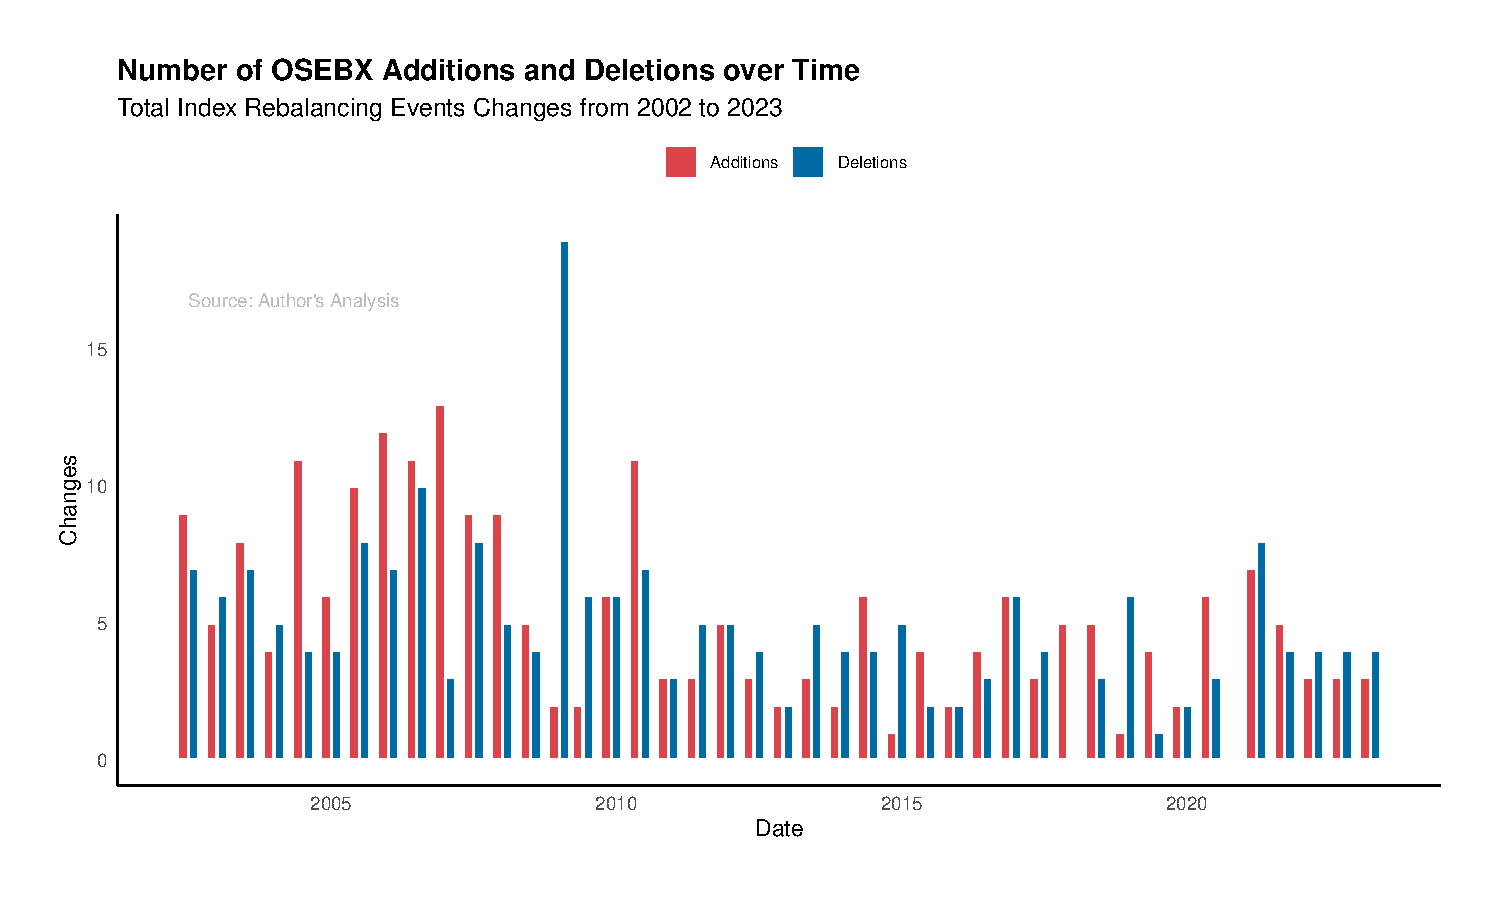
\includegraphics[width=1.06\textwidth]{images/plot_add_del.pdf}}
    \caption{{Number of OSEBX Additions and Deletions Over Time}}
    \subcaption*{Illustration of the number of additions and deletions to OSEBX in the period from 2002 to 2023. Typically, there are between 5-10 additions and deletions per index rebalancing event. We see quite a large number of deletions from OSEBX during the financial crisis.}
    \label{fig-OSEBX-Number-of-Additions-and-Deletions}
\end{figure}

The world saw its first index investing fund with John Bogle and the Vanguard 500 Index Fund in 1975 \parencite{vanguard-first-mutual-fund}. It was first of its kind in replicating a benchmark index and was mocked as Bogle's Folly. Since then, the fund has seen redemption by generating exceptional returns \parencite{vanguard-first-mutual-fund}. A benchmark index is a grouping of carefully selected assets, to represent the movement of the entire stock market \parencite{goel-index-tracking-and-enhanced-indexing-using-mixed-conditional-value-at-risk}. 

\textcite{afego-effects-of-changes-in-stock-index-composition} find differences in benchmark index transparency. The low transparency S\&P 500 has an undisclosed replacement pool and performs need-based rebalancing \parencite{afego-effects-of-changes-in-stock-index-composition}. OSEBX, on the other hand, is rebalanced twice a year and it uses the replacement pool Oslo Stock Exchange All Share Index (OSEAX). The OSEBX composition is determined by size and liquidity criteria, which is publicly available on the Euronext website \parencite{OSEBX-rule-book}. OSEBX is therefore considered to be relatively transparent \parencite{afego-effects-of-changes-in-stock-index-composition}. 

\textcite{financialtimes-active-to-passive} writes that money is pouring out of active funds and into passive, with passive assets under management (AUM) surpassing active AUM in the US. \textcite{morningstar-active-to-passive} find negative inflow to active funds for 7 of the last 10 years, with over \$250B inflow to passive funds in the same period. \textcite{jpmorgan-exchange-traded-funds-etfs} also found \$3T in flow from active to passive equity funds globally in the last 10 years.
 
 Passive index investing has increased in popularity, but it has also received criticism. \textcite{spglobal-the-slings-and-arrows-of-passive-fortune} state that "dangers of passive investing" turned up several times more than "dangers of passive smoking" on Google News results in 2018. Criticism of passive investing includes contributions to market bubbles and reduction in market efficiency \parencite{spglobal-the-slings-and-arrows-of-passive-fortune}. This rise of passive investing increases attention toward making enhancements by exploiting the index effect \parencite{elton-gruber-are-enhanced-index-funds-enhanced}.

The index effect may emerge from passive funds replicating benchmark indices \parencite{afego-effects-of-changes-in-stock-index-composition}. This can lead to price pressures around ED when the benchmark index changes its composition \parencite{investopedia-s&p-phenomenon}. If so, companies are not bought on good underlying information \parencite{federal-reserve-bank-is-there-an-s&p-500-index-effect}. \textcite{spglobal-what-happened-to-the-index-effect} find a revamping in the index effect amidst the trend towards passive investing. 

\textcite{nbim-investing-in-equities} has conducted enhancements to their index investing by exploiting the index effect. Using the benchmark index methodology, NBIM predicts and trades on additions and deletions \textit{at} the AD \parencite{nbim-investing-in-equities}. This strategy significantly boosted the returns of Norway's Government Pension Fund Global from 2000 to 2011 \parencite{ang-review-of-the-active-management-of-oljefondet}. Following enhancements, the fund may align more closely with an enhanced index fund than a purely passive one \parencite{døskeland-a-review-of-the-active-management-of-oljefondet}. 

Defining \textit{enhanced index investing} can be difficult \parencite{riepe-werner-are-enhanced-index-mutual-funds-worthy-of-their-name}. In relative terms, lower tracking error (TE) and higher returns are common characteristics \parencite{riepe-werner-are-enhanced-index-mutual-funds-worthy-of-their-name}. Enhancements to index investing, such as exploiting the index effect may justify the definition \parencite{goel-index-tracking-and-enhanced-indexing-using-mixed-conditional-value-at-risk}. \textcite{elton-gruber-are-enhanced-index-funds-enhanced} have found that making such enhancements can outperform passive index investing both for management ability (before costs), and investor returns (after costs). The last years have seen the emergence of global enhanced index funds \parencite{jp-morgan-enhanced-index}. Norway is starting to see this trend, with DNB Asset Management having started an enhanced index fund this October \parencite{dnb-global-enhanced-index}.

The existence of an index effect on OSEBX has been discussed in previous master's theses, but there is a lack of research on exploiting the index effect in practice. Furthermore, we have seen large investors make enhancements to index investing on large global indices, such as the S\&P 500, but not to the same extent on OSEBX. In this thesis, we seek to exploit the index effect on OSEBX in the most practical applied sense possible. We use ML to predict upcoming additions and deletions \textit{before} AD and simulate portfolios trading on these predictions. First, we simulate an active trading portfolio, and thereafter an enhanced index portfolio. We ask the following research questions:

\label{research-questions}
\begin{enumerate}
    \item \textit{To what degree can machine learning algorithms predict the index composition of OSEBX in the next period?}
    \item \textit{To what degree can trading on predicted additions and deletions outperform OSEBX in an active trading portfolio?}
    \item \textit{To what degree can trading on predicted additions and deletions outperform OSEBX in an enhanced index portfolio?}
\end{enumerate}

Next, the thesis includes a section on financial portfolio theory in \autoref{Theoretical background}, ML methodology used to predict index composition in \autoref{Methodology}, and an explanation of our data set for OSEAX companies in the period from 2006 to 2023 in \autoref{Data}. In \autoref{Results and discussion} we assess model performance, and present our findings from the portfolio simulations. Finally, we conclude the thesis in \autoref{Summary and conclusions}.    